\documentclass[12pt,a4paper,bibliography=totocnumbered,listof=totocnumbered]{scrartcl}
\usepackage[english]{babel}
\usepackage[utf8]{inputenc}
\usepackage{amsmath}
\usepackage{amsfonts}
\usepackage{amssymb}
\usepackage{graphicx}
\usepackage{fancyhdr}
\usepackage{tabularx}
\usepackage{geometry}
\usepackage{setspace}
\usepackage[right]{eurosym}
\usepackage[printonlyused]{acronym}
\usepackage{subfig}
\usepackage{floatflt}
\usepackage[usenames,dvipsnames]{color}
\usepackage{colortbl}
\usepackage{paralist}
\usepackage{array}
\usepackage{titlesec}
\usepackage{url}
%\usepackage{dsfont}
\usepackage{parskip}
\usepackage[right]{eurosym}
\usepackage[subfigure,titles]{tocloft}
\usepackage[pdfpagelabels=true]{hyperref}
\usepackage{hyperref}
\usepackage{mathdots}
\usepackage{listings}
\usepackage{lipsum}
\usepackage{booktabs}
\usepackage{fix-cm}
\usepackage{rotating}
\usepackage{pdflscape}
\usepackage[labelfont=bf]{caption}
\captionsetup{labelfont=bf}
\usepackage{tikz}
\usepackage{tocloft}
\usepackage{breakcites}
 \usepackage[flushleft]{threeparttable}
\renewcommand{\cftsecleader}{\cftdotfill{\cftdotsep}}
\usepackage{float}

\begin{document}

% ----------------------------------------------------------------------------------------------------------
% Front Page
% ----------------------------------------------------------------------------------------------------------

\thispagestyle{empty}
\begin{center}
	\includegraphics[width=\textwidth]{Pictures/logo01.jpg}\\
	\vspace*{2cm}
	\vspace*{2cm}
	\Huge
	\textbf{14D010 - TextMining for Social Sciences}\\
	\vspace*{0.5cm}
	\large
	\textbf{Final Project Report}\\
	\vspace*{1cm}
\end{center}	

$\vspace{6cm}$
\begin{tabbing}
	\hspace*{1cm}\=\hspace*{3.2cm}\=\hspace*{3cm}\=\hspace*{2.7cm}\= \kill
	\onehalfspacing
	\textbf{Author:} \>\> Felix Gutmann\\
	\textbf{Student number:} 	\>\> 125604\\
	\textbf{Program:} \>\> M.S. Data Science\\
	\textbf{E-Mail:} \>\> felix.gutmann@barcelonagse.eu
\end{tabbing}
\vspace{1cm}

% ----------------------------------------------------------------------------------------------------------
% Table of contents
% ----------------------------------------------------------------------------------------------------------
\renewcommand{\thesection}{\Roman{section}}
\renewcommand{\theHsection}{\Roman{section}}
\pagenumbering{Roman}
\titlespacing{\section}{0pt}{12pt plus 4pt minus 2pt}{2pt plus 2pt minus 2pt}
\singlespacing
\rhead{Table of contents}
\renewcommand{\contentsname}{I Table of Contents}
\phantomsection
\addcontentsline{toc}{section}{\texorpdfstring{I \hspace{0.35em}Table of Contents}{Table of Contents}}
\addtocounter{section}{1}
\setcounter{page}{1}

\pagenumbering{Roman}

\tableofcontents



% ----------------------------------------------------------------------------------------------------------
% List of figures
% ----------------------------------------------------------------------------------------------------------

\listoffigures

% ----------------------------------------------------------------------------------------------------------
% List of tables
% ----------------------------------------------------------------------------------------------------------

\listoftables

\pagebreak
% ----------------------------------------------------------------------------------------------------------
% Abstract
% ----------------------------------------------------------------------------------------------------------

\renewcommand{\thesection}{\arabic{section}}
\renewcommand{\theHsection}{\arabic{section}}
\setcounter{section}{0}
\pagenumbering{arabic}
\setcounter{page}{1}


\onehalfspacing
% ----------------------------------------------------------------------------------------------------------
% Section 1 - Introduction
% ----------------------------------------------------------------------------------------------------------

\section{Introduction}

Musical work has both a acoustic and lyrical component. This paper aims to evaluate the application possibilities of text data on identifying successful songs. A natural way of measuring success is by considering monetary success. However, precise information on sales data are not  immediately available. A more modern indicator of success would be to consider streaming data (e.g. Spotify or YouTube). Gathering those might be feasible, but the time expense of this process might disproportional to the scope of the project. \\
Based on revenues some singles (or LPs) are awarded with golden or even platinum records. An advantage of those awards is that they a more  time independent, because the awarding criteria got adjusted constantly over the years.
Based on that the objective is to find out if the lyrics can be processed and used in such a way that they can be used to predict awards for a given song using several unsupervised learning algorithms. The underlying data for this projects consists of lyrics of the yearly final chart entries of the Billboard Hot-100 single chars and related awards for each song (see in more detail later on). The time frame considered in this project is from 2000 to 2015. \\
The report has the following structure. In section two the data gathering process is outlined. Additionally, this section involves an outline of the data pre-processing and a summary of the resulting final data set.\\
Section three is dedicated to the analysis. First there is a small introduction of the subsequently applied classifiers. This is especially dedicated to random forest classifier. Data in a text mining context are usually high dimensional. Hence, this section also  involves a short discussion how features are selected to find a adequate model. To boost predictive power some additional feature extracted from the lyrics are also outlined. This section closes with a summary of prediction results.
Finally the papers closes by summarizing results and some critical remarks.


\section{Data; Collection, processing and summary}

This section is dedicated to the data collection process. This involves also a short outline of related problems.\\ 
The data for this project come from three different websites. \cite{wiki} provides a yearly overview of the yearly \href{https://en.wikipedia.org/wiki/Billboard_Year-End_Hot_100_singles_of_2015}{Billboard Hot 100} closing single charts. It is listing the most successful singles of a given year (based revenues). Information on chart position, artist and song title got scrapped from this source.These information are used to get the remaining data. \\ 
For the lyrics \cite{songlyrics} serves as an appropriate data source. Signed up users can comment and enter lyrics. It is just one of plenty options, but the site has a nice and clean structure, which makes it fairly easy to scrape. Some lyrics failed to scrape, mostly due to artist spelling. No uniform pattern could be identified to automatize those exceptions, so they were ignored (more details are provided in the data summary later on). \\
Finally, The awards come from \cite{riaa}. They award golden, or platinum record as a benchmark for success. There a certain criteria, which have to be fulfilled to be awarded. Superficially spoken records have to generate a certain amount of revenue.\footnote{There is a more detailed system how much for example digital units or records contribute to revenue or additional extras in collectors editions. A more detailed breakdown can be found on \cite{riaa}.}\\
The categories are ordinal, meaning when single is awarded with platinum it also got awarded with a gold record. In the following a song solely belongs to the highest achieved award. Furthermore, a single can get multiple platinum records. For example the latest Rihanna song "Work" has already three platinum awards. Those cases are also not considered in this project. A single can only belong to either one of the three categories; \textit{"no award"}, \textit{"gold"} or \textit{"platinum"}.
Finally table \ref{tab:ov} summarizes the three data sources and related data

\begin{table}[H]
	\centering
	\small
	\begin{tabular}{l l}
		\toprule 
		\textbf{Website} & \textbf{Content} \\
		\hline
		Wikipedia.org & Yearly charts artists and song titles \\
		songlyrics.com & Lyrics for each scraped song \\
		Riaa.com & Information about award	\\
		\bottomrule
	\end{tabular}
	\caption{Overview of data sources}
	\label{tab:ov}
\end{table}

For 15 years we should find 1500 songs. However, the sample got reduced due to several reasons. First, 33 singles and 83 lyrics could not be scrapped, mostly due to special artist spelling. A unique pattern could not be identified and hence a subsequent manual scrape was not performed.\\
Furthermore, one can observe that some songs are in Spanish. Those got removed from the data, because the would have to be processed individually. With four songs the number of removed songs was quite moderate.\footnote{The language got detect with langdetect library. A simple approach using Spanish stop words turned out to be not reliable enough}\\ 
The remaining text got processed in the following standardized way. Non alpha numeric characters got filtered from the text. In the next step stop words got removed.\footnote{The stop word list comes from the natural language toolkit library (nltk)}After browsing the resulting lyrics, further adjustments were necessary. For example a lot of lyrics contain small words like "oh" or "ah" with a high frequency. Obviously, they are not contributing to the analysis at all. Hence, all words with length less than three got also removed. Finally, the tokens for each document got stemmed with a porter stemmer.\footnote{ This also come from nltk library}. Based on this the term document matrix got computed.\\

Table \ref{tab:summary} gives a summary of the final data set. We can observe that the class of platinum records is oversampled while gold records are under sampled. This makes  sense since platinum records also include gold awards.

\begin{table}[H]
	\centering
	\footnotesize
	\begin{tabular}{l r l}
		\toprule 
		\textbf{Indicator} & \textbf{Value} & \textbf{Ratio} \\
		\hline
		Number of observations & 1,380 & -\\
		Number of distinct artists & 521  & - \\
		Number of unique stemmed terms in corpus & 9.585 & -  \\
		Number of distinct stemmed terms per document & 86.55 & - \\
		Single records with no awards & 499  &  36.16  \\
		Singles records with gold awards & 208  & 15.07  \\
		Singles records with platinum awards & 673 & 48.77 \\
		\bottomrule 
	\end{tabular}
		\caption{Data Summary - Yearly Billboard Hot 100 (Cleaned, 2000 - 2015)}
		\label{tab:summary}
\end{table}
\pagebreak

Figure \ref{fig:fig1} depicts the artist - award distribution. Sug-figure \ref{fig:fig1} (a) shows the number of awards and corresponding frequency for each of the three categories in the data set. We can observe that all three follow roughly a power law distribution. Sub figure (b) illustrates top 5 five artist in the tail based on the most frequent appearance. We see that those artist are rather really high or non awarded.

\begin{figure}[H]
	\centering
				\small
	\begingroup
	\hspace*{-1.5in}
	\tikzset{every picture/.style={scale=1}}
	\begin{tabular}{p{7cm}p{7cm}}
	% Created by tikzDevice version 0.10.1 on 2016-06-26 23:09:38
% !TEX encoding = UTF-8 Unicode
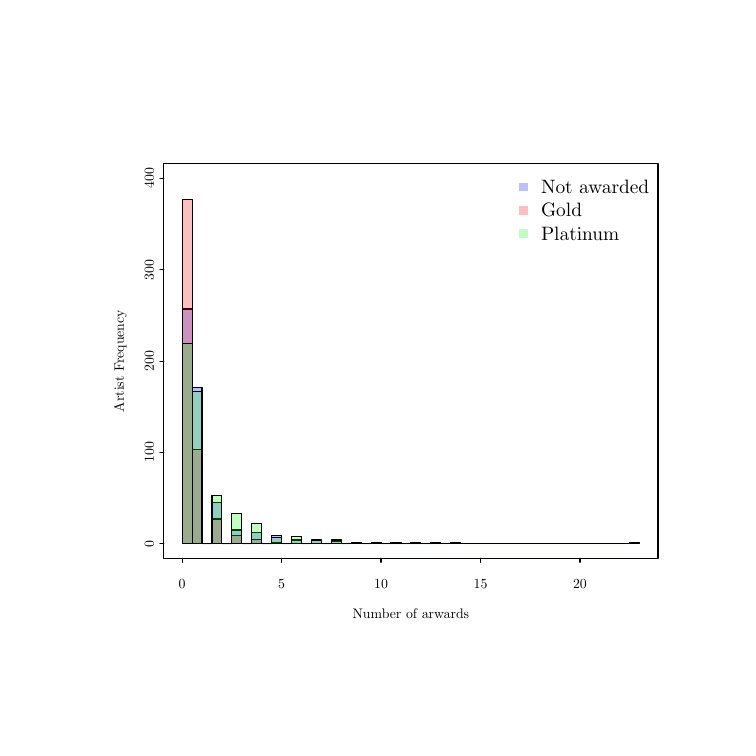
\begin{tikzpicture}[x=1pt,y=1pt]
\definecolor{fillColor}{RGB}{255,255,255}
\path[use as bounding box,fill=fillColor,fill opacity=0.00] (0,0) rectangle (252.94,252.94);
\begin{scope}
\path[clip] (  0.00,  0.00) rectangle (252.94,252.94);
\definecolor{drawColor}{RGB}{0,0,0}

\node[text=drawColor,anchor=base,inner sep=0pt, outer sep=0pt, scale=  0.50] at (138.47, 39.60) {Number of arwards};

\node[text=drawColor,rotate= 90.00,anchor=base,inner sep=0pt, outer sep=0pt, scale=  0.50] at ( 34.80,132.47) {Artist Frequency};
\end{scope}
\begin{scope}
\path[clip] (  0.00,  0.00) rectangle (252.94,252.94);
\definecolor{drawColor}{RGB}{0,0,0}

\path[draw=drawColor,line width= 0.4pt,line join=round,line cap=round] ( 55.81, 61.20) -- (199.57, 61.20);

\path[draw=drawColor,line width= 0.4pt,line join=round,line cap=round] ( 55.81, 61.20) -- ( 55.81, 59.77);

\path[draw=drawColor,line width= 0.4pt,line join=round,line cap=round] ( 91.75, 61.20) -- ( 91.75, 59.77);

\path[draw=drawColor,line width= 0.4pt,line join=round,line cap=round] (127.69, 61.20) -- (127.69, 59.77);

\path[draw=drawColor,line width= 0.4pt,line join=round,line cap=round] (163.63, 61.20) -- (163.63, 59.77);

\path[draw=drawColor,line width= 0.4pt,line join=round,line cap=round] (199.57, 61.20) -- (199.57, 59.77);

\node[text=drawColor,anchor=base,inner sep=0pt, outer sep=0pt, scale=  0.50] at ( 55.81, 50.40) {0};

\node[text=drawColor,anchor=base,inner sep=0pt, outer sep=0pt, scale=  0.50] at ( 91.75, 50.40) {5};

\node[text=drawColor,anchor=base,inner sep=0pt, outer sep=0pt, scale=  0.50] at (127.69, 50.40) {10};

\node[text=drawColor,anchor=base,inner sep=0pt, outer sep=0pt, scale=  0.50] at (163.63, 50.40) {15};

\node[text=drawColor,anchor=base,inner sep=0pt, outer sep=0pt, scale=  0.50] at (199.57, 50.40) {20};

\path[draw=drawColor,line width= 0.4pt,line join=round,line cap=round] ( 49.20, 66.48) -- ( 49.20,198.47);

\path[draw=drawColor,line width= 0.4pt,line join=round,line cap=round] ( 49.20, 66.48) -- ( 47.77, 66.48);

\path[draw=drawColor,line width= 0.4pt,line join=round,line cap=round] ( 49.20, 99.48) -- ( 47.77, 99.48);

\path[draw=drawColor,line width= 0.4pt,line join=round,line cap=round] ( 49.20,132.47) -- ( 47.77,132.47);

\path[draw=drawColor,line width= 0.4pt,line join=round,line cap=round] ( 49.20,165.47) -- ( 47.77,165.47);

\path[draw=drawColor,line width= 0.4pt,line join=round,line cap=round] ( 49.20,198.47) -- ( 47.77,198.47);

\node[text=drawColor,rotate= 90.00,anchor=base,inner sep=0pt, outer sep=0pt, scale=  0.50] at ( 45.60, 66.48) {0};

\node[text=drawColor,rotate= 90.00,anchor=base,inner sep=0pt, outer sep=0pt, scale=  0.50] at ( 45.60, 99.48) {100};

\node[text=drawColor,rotate= 90.00,anchor=base,inner sep=0pt, outer sep=0pt, scale=  0.50] at ( 45.60,132.47) {200};

\node[text=drawColor,rotate= 90.00,anchor=base,inner sep=0pt, outer sep=0pt, scale=  0.50] at ( 45.60,165.47) {300};

\node[text=drawColor,rotate= 90.00,anchor=base,inner sep=0pt, outer sep=0pt, scale=  0.50] at ( 45.60,198.47) {400};
\end{scope}
\begin{scope}
\path[clip] ( 49.20, 61.20) rectangle (227.75,203.75);
\definecolor{drawColor}{RGB}{0,0,0}
\definecolor{fillColor}{RGB}{0,0,255}

\path[draw=drawColor,line width= 0.4pt,line join=round,line cap=round,fill=fillColor,fill opacity=0.25] ( 55.81, 66.48) rectangle ( 59.41,151.28);

\path[draw=drawColor,line width= 0.4pt,line join=round,line cap=round,fill=fillColor,fill opacity=0.25] ( 59.41, 66.48) rectangle ( 63.00,122.90);

\path[draw=drawColor,line width= 0.4pt,line join=round,line cap=round,fill=fillColor,fill opacity=0.25] ( 63.00, 66.48) rectangle ( 66.59, 66.48);

\path[draw=drawColor,line width= 0.4pt,line join=round,line cap=round,fill=fillColor,fill opacity=0.25] ( 66.59, 66.48) rectangle ( 70.19, 81.33);

\path[draw=drawColor,line width= 0.4pt,line join=round,line cap=round,fill=fillColor,fill opacity=0.25] ( 70.19, 66.48) rectangle ( 73.78, 66.48);

\path[draw=drawColor,line width= 0.4pt,line join=round,line cap=round,fill=fillColor,fill opacity=0.25] ( 73.78, 66.48) rectangle ( 77.38, 71.43);

\path[draw=drawColor,line width= 0.4pt,line join=round,line cap=round,fill=fillColor,fill opacity=0.25] ( 77.38, 66.48) rectangle ( 80.97, 66.48);

\path[draw=drawColor,line width= 0.4pt,line join=round,line cap=round,fill=fillColor,fill opacity=0.25] ( 80.97, 66.48) rectangle ( 84.56, 70.44);

\path[draw=drawColor,line width= 0.4pt,line join=round,line cap=round,fill=fillColor,fill opacity=0.25] ( 84.56, 66.48) rectangle ( 88.16, 66.48);

\path[draw=drawColor,line width= 0.4pt,line join=round,line cap=round,fill=fillColor,fill opacity=0.25] ( 88.16, 66.48) rectangle ( 91.75, 69.45);

\path[draw=drawColor,line width= 0.4pt,line join=round,line cap=round,fill=fillColor,fill opacity=0.25] ( 91.75, 66.48) rectangle ( 95.35, 66.48);

\path[draw=drawColor,line width= 0.4pt,line join=round,line cap=round,fill=fillColor,fill opacity=0.25] ( 95.35, 66.48) rectangle ( 98.94, 67.80);

\path[draw=drawColor,line width= 0.4pt,line join=round,line cap=round,fill=fillColor,fill opacity=0.25] ( 98.94, 66.48) rectangle (102.53, 66.48);

\path[draw=drawColor,line width= 0.4pt,line join=round,line cap=round,fill=fillColor,fill opacity=0.25] (102.53, 66.48) rectangle (106.13, 67.80);

\path[draw=drawColor,line width= 0.4pt,line join=round,line cap=round,fill=fillColor,fill opacity=0.25] (106.13, 66.48) rectangle (109.72, 66.48);

\path[draw=drawColor,line width= 0.4pt,line join=round,line cap=round,fill=fillColor,fill opacity=0.25] (109.72, 66.48) rectangle (113.32, 67.14);

\path[draw=drawColor,line width= 0.4pt,line join=round,line cap=round,fill=fillColor,fill opacity=0.25] (113.32, 66.48) rectangle (116.91, 66.48);

\path[draw=drawColor,line width= 0.4pt,line join=round,line cap=round,fill=fillColor,fill opacity=0.25] (116.91, 66.48) rectangle (120.50, 66.81);

\path[draw=drawColor,line width= 0.4pt,line join=round,line cap=round,fill=fillColor,fill opacity=0.25] (120.50, 66.48) rectangle (124.10, 66.48);

\path[draw=drawColor,line width= 0.4pt,line join=round,line cap=round,fill=fillColor,fill opacity=0.25] (124.10, 66.48) rectangle (127.69, 66.81);

\path[draw=drawColor,line width= 0.4pt,line join=round,line cap=round,fill=fillColor,fill opacity=0.25] (127.69, 66.48) rectangle (131.28, 66.48);

\path[draw=drawColor,line width= 0.4pt,line join=round,line cap=round,fill=fillColor,fill opacity=0.25] (131.28, 66.48) rectangle (134.88, 66.48);

\path[draw=drawColor,line width= 0.4pt,line join=round,line cap=round,fill=fillColor,fill opacity=0.25] (134.88, 66.48) rectangle (138.47, 66.48);

\path[draw=drawColor,line width= 0.4pt,line join=round,line cap=round,fill=fillColor,fill opacity=0.25] (138.47, 66.48) rectangle (142.07, 66.48);

\path[draw=drawColor,line width= 0.4pt,line join=round,line cap=round,fill=fillColor,fill opacity=0.25] (142.07, 66.48) rectangle (145.66, 66.48);

\path[draw=drawColor,line width= 0.4pt,line join=round,line cap=round,fill=fillColor,fill opacity=0.25] (145.66, 66.48) rectangle (149.25, 66.81);
\definecolor{fillColor}{RGB}{255,0,0}

\path[draw=drawColor,line width= 0.4pt,line join=round,line cap=round,fill=fillColor,fill opacity=0.25] ( 55.81, 66.48) rectangle ( 59.41,190.88);

\path[draw=drawColor,line width= 0.4pt,line join=round,line cap=round,fill=fillColor,fill opacity=0.25] ( 59.41, 66.48) rectangle ( 63.00,100.47);

\path[draw=drawColor,line width= 0.4pt,line join=round,line cap=round,fill=fillColor,fill opacity=0.25] ( 63.00, 66.48) rectangle ( 66.59, 66.48);

\path[draw=drawColor,line width= 0.4pt,line join=round,line cap=round,fill=fillColor,fill opacity=0.25] ( 66.59, 66.48) rectangle ( 70.19, 75.39);

\path[draw=drawColor,line width= 0.4pt,line join=round,line cap=round,fill=fillColor,fill opacity=0.25] ( 70.19, 66.48) rectangle ( 73.78, 66.48);

\path[draw=drawColor,line width= 0.4pt,line join=round,line cap=round,fill=fillColor,fill opacity=0.25] ( 73.78, 66.48) rectangle ( 77.38, 69.45);

\path[draw=drawColor,line width= 0.4pt,line join=round,line cap=round,fill=fillColor,fill opacity=0.25] ( 77.38, 66.48) rectangle ( 80.97, 66.48);

\path[draw=drawColor,line width= 0.4pt,line join=round,line cap=round,fill=fillColor,fill opacity=0.25] ( 80.97, 66.48) rectangle ( 84.56, 68.13);

\path[draw=drawColor,line width= 0.4pt,line join=round,line cap=round,fill=fillColor,fill opacity=0.25] ( 84.56, 66.48) rectangle ( 88.16, 66.48);

\path[draw=drawColor,line width= 0.4pt,line join=round,line cap=round,fill=fillColor,fill opacity=0.25] ( 88.16, 66.48) rectangle ( 91.75, 66.81);
\definecolor{fillColor}{RGB}{0,255,0}

\path[draw=drawColor,line width= 0.4pt,line join=round,line cap=round,fill=fillColor,fill opacity=0.25] ( 55.81, 66.48) rectangle ( 59.41,138.74);

\path[draw=drawColor,line width= 0.4pt,line join=round,line cap=round,fill=fillColor,fill opacity=0.25] ( 59.41, 66.48) rectangle ( 63.00,121.58);

\path[draw=drawColor,line width= 0.4pt,line join=round,line cap=round,fill=fillColor,fill opacity=0.25] ( 63.00, 66.48) rectangle ( 66.59, 66.48);

\path[draw=drawColor,line width= 0.4pt,line join=round,line cap=round,fill=fillColor,fill opacity=0.25] ( 66.59, 66.48) rectangle ( 70.19, 83.97);

\path[draw=drawColor,line width= 0.4pt,line join=round,line cap=round,fill=fillColor,fill opacity=0.25] ( 70.19, 66.48) rectangle ( 73.78, 66.48);

\path[draw=drawColor,line width= 0.4pt,line join=round,line cap=round,fill=fillColor,fill opacity=0.25] ( 73.78, 66.48) rectangle ( 77.38, 77.37);

\path[draw=drawColor,line width= 0.4pt,line join=round,line cap=round,fill=fillColor,fill opacity=0.25] ( 77.38, 66.48) rectangle ( 80.97, 66.48);

\path[draw=drawColor,line width= 0.4pt,line join=round,line cap=round,fill=fillColor,fill opacity=0.25] ( 80.97, 66.48) rectangle ( 84.56, 73.74);

\path[draw=drawColor,line width= 0.4pt,line join=round,line cap=round,fill=fillColor,fill opacity=0.25] ( 84.56, 66.48) rectangle ( 88.16, 66.48);

\path[draw=drawColor,line width= 0.4pt,line join=round,line cap=round,fill=fillColor,fill opacity=0.25] ( 88.16, 66.48) rectangle ( 91.75, 68.79);

\path[draw=drawColor,line width= 0.4pt,line join=round,line cap=round,fill=fillColor,fill opacity=0.25] ( 91.75, 66.48) rectangle ( 95.35, 66.48);

\path[draw=drawColor,line width= 0.4pt,line join=round,line cap=round,fill=fillColor,fill opacity=0.25] ( 95.35, 66.48) rectangle ( 98.94, 69.12);

\path[draw=drawColor,line width= 0.4pt,line join=round,line cap=round,fill=fillColor,fill opacity=0.25] ( 98.94, 66.48) rectangle (102.53, 66.48);

\path[draw=drawColor,line width= 0.4pt,line join=round,line cap=round,fill=fillColor,fill opacity=0.25] (102.53, 66.48) rectangle (106.13, 67.47);

\path[draw=drawColor,line width= 0.4pt,line join=round,line cap=round,fill=fillColor,fill opacity=0.25] (106.13, 66.48) rectangle (109.72, 66.48);

\path[draw=drawColor,line width= 0.4pt,line join=round,line cap=round,fill=fillColor,fill opacity=0.25] (109.72, 66.48) rectangle (113.32, 67.80);

\path[draw=drawColor,line width= 0.4pt,line join=round,line cap=round,fill=fillColor,fill opacity=0.25] (113.32, 66.48) rectangle (116.91, 66.48);

\path[draw=drawColor,line width= 0.4pt,line join=round,line cap=round,fill=fillColor,fill opacity=0.25] (116.91, 66.48) rectangle (120.50, 66.81);

\path[draw=drawColor,line width= 0.4pt,line join=round,line cap=round,fill=fillColor,fill opacity=0.25] (120.50, 66.48) rectangle (124.10, 66.48);

\path[draw=drawColor,line width= 0.4pt,line join=round,line cap=round,fill=fillColor,fill opacity=0.25] (124.10, 66.48) rectangle (127.69, 66.81);

\path[draw=drawColor,line width= 0.4pt,line join=round,line cap=round,fill=fillColor,fill opacity=0.25] (127.69, 66.48) rectangle (131.28, 66.48);

\path[draw=drawColor,line width= 0.4pt,line join=round,line cap=round,fill=fillColor,fill opacity=0.25] (131.28, 66.48) rectangle (134.88, 66.81);

\path[draw=drawColor,line width= 0.4pt,line join=round,line cap=round,fill=fillColor,fill opacity=0.25] (134.88, 66.48) rectangle (138.47, 66.48);

\path[draw=drawColor,line width= 0.4pt,line join=round,line cap=round,fill=fillColor,fill opacity=0.25] (138.47, 66.48) rectangle (142.07, 66.81);

\path[draw=drawColor,line width= 0.4pt,line join=round,line cap=round,fill=fillColor,fill opacity=0.25] (142.07, 66.48) rectangle (145.66, 66.48);

\path[draw=drawColor,line width= 0.4pt,line join=round,line cap=round,fill=fillColor,fill opacity=0.25] (145.66, 66.48) rectangle (149.25, 66.48);

\path[draw=drawColor,line width= 0.4pt,line join=round,line cap=round,fill=fillColor,fill opacity=0.25] (149.25, 66.48) rectangle (152.85, 66.48);

\path[draw=drawColor,line width= 0.4pt,line join=round,line cap=round,fill=fillColor,fill opacity=0.25] (152.85, 66.48) rectangle (156.44, 66.81);

\path[draw=drawColor,line width= 0.4pt,line join=round,line cap=round,fill=fillColor,fill opacity=0.25] (156.44, 66.48) rectangle (160.04, 66.48);

\path[draw=drawColor,line width= 0.4pt,line join=round,line cap=round,fill=fillColor,fill opacity=0.25] (160.04, 66.48) rectangle (163.63, 66.48);

\path[draw=drawColor,line width= 0.4pt,line join=round,line cap=round,fill=fillColor,fill opacity=0.25] (163.63, 66.48) rectangle (167.22, 66.48);

\path[draw=drawColor,line width= 0.4pt,line join=round,line cap=round,fill=fillColor,fill opacity=0.25] (167.22, 66.48) rectangle (170.82, 66.48);

\path[draw=drawColor,line width= 0.4pt,line join=round,line cap=round,fill=fillColor,fill opacity=0.25] (170.82, 66.48) rectangle (174.41, 66.48);

\path[draw=drawColor,line width= 0.4pt,line join=round,line cap=round,fill=fillColor,fill opacity=0.25] (174.41, 66.48) rectangle (178.01, 66.48);

\path[draw=drawColor,line width= 0.4pt,line join=round,line cap=round,fill=fillColor,fill opacity=0.25] (178.01, 66.48) rectangle (181.60, 66.48);

\path[draw=drawColor,line width= 0.4pt,line join=round,line cap=round,fill=fillColor,fill opacity=0.25] (181.60, 66.48) rectangle (185.19, 66.48);

\path[draw=drawColor,line width= 0.4pt,line join=round,line cap=round,fill=fillColor,fill opacity=0.25] (185.19, 66.48) rectangle (188.79, 66.48);

\path[draw=drawColor,line width= 0.4pt,line join=round,line cap=round,fill=fillColor,fill opacity=0.25] (188.79, 66.48) rectangle (192.38, 66.48);

\path[draw=drawColor,line width= 0.4pt,line join=round,line cap=round,fill=fillColor,fill opacity=0.25] (192.38, 66.48) rectangle (195.97, 66.48);

\path[draw=drawColor,line width= 0.4pt,line join=round,line cap=round,fill=fillColor,fill opacity=0.25] (195.97, 66.48) rectangle (199.57, 66.48);

\path[draw=drawColor,line width= 0.4pt,line join=round,line cap=round,fill=fillColor,fill opacity=0.25] (199.57, 66.48) rectangle (203.16, 66.48);

\path[draw=drawColor,line width= 0.4pt,line join=round,line cap=round,fill=fillColor,fill opacity=0.25] (203.16, 66.48) rectangle (206.76, 66.48);

\path[draw=drawColor,line width= 0.4pt,line join=round,line cap=round,fill=fillColor,fill opacity=0.25] (206.76, 66.48) rectangle (210.35, 66.48);

\path[draw=drawColor,line width= 0.4pt,line join=round,line cap=round,fill=fillColor,fill opacity=0.25] (210.35, 66.48) rectangle (213.94, 66.48);

\path[draw=drawColor,line width= 0.4pt,line join=round,line cap=round,fill=fillColor,fill opacity=0.25] (213.94, 66.48) rectangle (217.54, 66.48);

\path[draw=drawColor,line width= 0.4pt,line join=round,line cap=round,fill=fillColor,fill opacity=0.25] (217.54, 66.48) rectangle (221.13, 66.81);
\definecolor{fillColor}{RGB}{0,0,255}

\path[fill=fillColor,fill opacity=0.25] (177.63,193.77) --
	(180.78,193.77) --
	(180.78,196.92) --
	(177.63,196.92) --
	cycle;
\definecolor{fillColor}{RGB}{255,0,0}

\path[fill=fillColor,fill opacity=0.25] (177.63,185.37) --
	(180.78,185.37) --
	(180.78,188.52) --
	(177.63,188.52) --
	cycle;
\definecolor{fillColor}{RGB}{0,255,0}

\path[fill=fillColor,fill opacity=0.25] (177.63,176.97) --
	(180.78,176.97) --
	(180.78,180.12) --
	(177.63,180.12) --
	cycle;

\node[text=drawColor,anchor=base west,inner sep=0pt, outer sep=0pt, scale=  0.70] at (185.50,192.93) {Not awarded};

\node[text=drawColor,anchor=base west,inner sep=0pt, outer sep=0pt, scale=  0.70] at (185.50,184.53) {Gold};

\node[text=drawColor,anchor=base west,inner sep=0pt, outer sep=0pt, scale=  0.70] at (185.50,176.13) {Platinum};
\end{scope}
\begin{scope}
\path[clip] (  0.00,  0.00) rectangle (252.94,252.94);
\definecolor{drawColor}{RGB}{0,0,0}

\path[draw=drawColor,line width= 0.4pt,line join=round,line cap=round] ( 49.20, 61.20) --
	(227.75, 61.20) --
	(227.75,203.75) --
	( 49.20,203.75) --
	( 49.20, 61.20);
\end{scope}
\end{tikzpicture}
 & % Created by tikzDevice version 0.10.1 on 2016-06-26 23:06:37
% !TEX encoding = UTF-8 Unicode
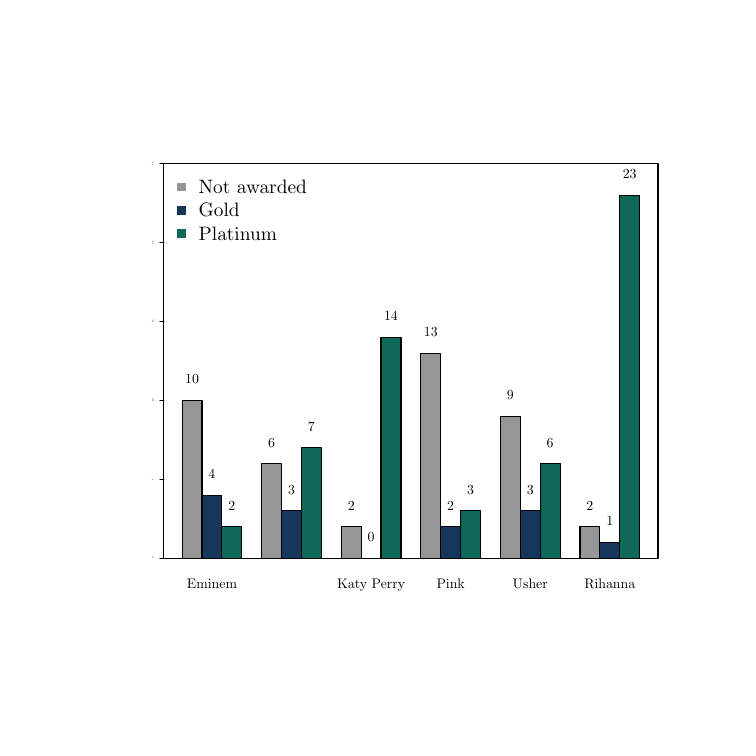
\begin{tikzpicture}[x=1pt,y=1pt]
\definecolor{fillColor}{RGB}{255,255,255}
\path[use as bounding box,fill=fillColor,fill opacity=0.00] (0,0) rectangle (252.94,252.94);
\begin{scope}
\path[clip] (  0.00,  0.00) rectangle (252.94,252.94);
\definecolor{drawColor}{RGB}{0,0,0}
\definecolor{fillColor}{gray}{0.59}

\path[draw=drawColor,line width= 0.4pt,line join=round,line cap=round,fill=fillColor] ( 55.81, 61.20) rectangle ( 63.00,118.22);
\definecolor{fillColor}{RGB}{22,54,92}

\path[draw=drawColor,line width= 0.4pt,line join=round,line cap=round,fill=fillColor] ( 63.00, 61.20) rectangle ( 70.19, 84.01);
\definecolor{fillColor}{RGB}{14,105,90}

\path[draw=drawColor,line width= 0.4pt,line join=round,line cap=round,fill=fillColor] ( 70.19, 61.20) rectangle ( 77.38, 72.60);
\definecolor{fillColor}{gray}{0.59}

\path[draw=drawColor,line width= 0.4pt,line join=round,line cap=round,fill=fillColor] ( 84.56, 61.20) rectangle ( 91.75, 95.41);
\definecolor{fillColor}{RGB}{22,54,92}

\path[draw=drawColor,line width= 0.4pt,line join=round,line cap=round,fill=fillColor] ( 91.75, 61.20) rectangle ( 98.94, 78.31);
\definecolor{fillColor}{RGB}{14,105,90}

\path[draw=drawColor,line width= 0.4pt,line join=round,line cap=round,fill=fillColor] ( 98.94, 61.20) rectangle (106.13,101.11);
\definecolor{fillColor}{gray}{0.59}

\path[draw=drawColor,line width= 0.4pt,line join=round,line cap=round,fill=fillColor] (113.32, 61.20) rectangle (120.50, 72.60);
\definecolor{fillColor}{RGB}{22,54,92}

\path[draw=drawColor,line width= 0.4pt,line join=round,line cap=round,fill=fillColor] (120.50, 61.20) rectangle (127.69, 61.20);
\definecolor{fillColor}{RGB}{14,105,90}

\path[draw=drawColor,line width= 0.4pt,line join=round,line cap=round,fill=fillColor] (127.69, 61.20) rectangle (134.88,141.03);
\definecolor{fillColor}{gray}{0.59}

\path[draw=drawColor,line width= 0.4pt,line join=round,line cap=round,fill=fillColor] (142.07, 61.20) rectangle (149.25,135.32);
\definecolor{fillColor}{RGB}{22,54,92}

\path[draw=drawColor,line width= 0.4pt,line join=round,line cap=round,fill=fillColor] (149.25, 61.20) rectangle (156.44, 72.60);
\definecolor{fillColor}{RGB}{14,105,90}

\path[draw=drawColor,line width= 0.4pt,line join=round,line cap=round,fill=fillColor] (156.44, 61.20) rectangle (163.63, 78.31);
\definecolor{fillColor}{gray}{0.59}

\path[draw=drawColor,line width= 0.4pt,line join=round,line cap=round,fill=fillColor] (170.82, 61.20) rectangle (178.01,112.52);
\definecolor{fillColor}{RGB}{22,54,92}

\path[draw=drawColor,line width= 0.4pt,line join=round,line cap=round,fill=fillColor] (178.01, 61.20) rectangle (185.19, 78.31);
\definecolor{fillColor}{RGB}{14,105,90}

\path[draw=drawColor,line width= 0.4pt,line join=round,line cap=round,fill=fillColor] (185.19, 61.20) rectangle (192.38, 95.41);
\definecolor{fillColor}{gray}{0.59}

\path[draw=drawColor,line width= 0.4pt,line join=round,line cap=round,fill=fillColor] (199.57, 61.20) rectangle (206.76, 72.60);
\definecolor{fillColor}{RGB}{22,54,92}

\path[draw=drawColor,line width= 0.4pt,line join=round,line cap=round,fill=fillColor] (206.76, 61.20) rectangle (213.94, 66.90);
\definecolor{fillColor}{RGB}{14,105,90}

\path[draw=drawColor,line width= 0.4pt,line join=round,line cap=round,fill=fillColor] (213.94, 61.20) rectangle (221.13,192.34);
\end{scope}
\begin{scope}
\path[clip] (  0.00,  0.00) rectangle (252.94,252.94);
\definecolor{drawColor}{RGB}{0,0,0}

\node[text=drawColor,anchor=base,inner sep=0pt, outer sep=0pt, scale=  0.50] at ( 66.59, 50.40) {Eminem};

\node[text=drawColor,anchor=base,inner sep=0pt, outer sep=0pt, scale=  0.50] at (124.10, 50.40) {Katy Perry};

\node[text=drawColor,anchor=base,inner sep=0pt, outer sep=0pt, scale=  0.50] at (152.85, 50.40) {Pink };

\node[text=drawColor,anchor=base,inner sep=0pt, outer sep=0pt, scale=  0.50] at (181.60, 50.40) {Usher };

\node[text=drawColor,anchor=base,inner sep=0pt, outer sep=0pt, scale=  0.50] at (210.35, 50.40) {Rihanna};

\path[draw=drawColor,line width= 0.4pt,line join=round,line cap=round] ( 49.20, 61.20) -- ( 49.20,203.75);

\path[draw=drawColor,line width= 0.4pt,line join=round,line cap=round] ( 49.20, 61.20) -- ( 47.77, 61.20);

\path[draw=drawColor,line width= 0.4pt,line join=round,line cap=round] ( 49.20, 89.71) -- ( 47.77, 89.71);

\path[draw=drawColor,line width= 0.4pt,line join=round,line cap=round] ( 49.20,118.22) -- ( 47.77,118.22);

\path[draw=drawColor,line width= 0.4pt,line join=round,line cap=round] ( 49.20,146.73) -- ( 47.77,146.73);

\path[draw=drawColor,line width= 0.4pt,line join=round,line cap=round] ( 49.20,175.24) -- ( 47.77,175.24);

\path[draw=drawColor,line width= 0.4pt,line join=round,line cap=round] ( 49.20,203.75) -- ( 47.77,203.75);

\node[text=drawColor,rotate= 90.00,anchor=base,inner sep=0pt, outer sep=0pt, scale=  0.10] at ( 45.60, 61.20) {0};

\node[text=drawColor,rotate= 90.00,anchor=base,inner sep=0pt, outer sep=0pt, scale=  0.10] at ( 45.60, 89.71) {5};

\node[text=drawColor,rotate= 90.00,anchor=base,inner sep=0pt, outer sep=0pt, scale=  0.10] at ( 45.60,118.22) {10};

\node[text=drawColor,rotate= 90.00,anchor=base,inner sep=0pt, outer sep=0pt, scale=  0.10] at ( 45.60,146.73) {15};

\node[text=drawColor,rotate= 90.00,anchor=base,inner sep=0pt, outer sep=0pt, scale=  0.10] at ( 45.60,175.24) {20};

\node[text=drawColor,rotate= 90.00,anchor=base,inner sep=0pt, outer sep=0pt, scale=  0.10] at ( 45.60,203.75) {25};
\end{scope}
\begin{scope}
\path[clip] ( 49.20, 61.20) rectangle (227.75,203.75);
\definecolor{drawColor}{RGB}{0,0,0}

\node[text=drawColor,anchor=base,inner sep=0pt, outer sep=0pt, scale=  0.50] at ( 59.41,124.22) {10};

\node[text=drawColor,anchor=base,inner sep=0pt, outer sep=0pt, scale=  0.50] at ( 66.59, 90.01) {4};

\node[text=drawColor,anchor=base,inner sep=0pt, outer sep=0pt, scale=  0.50] at ( 73.78, 78.60) {2};

\node[text=drawColor,anchor=base,inner sep=0pt, outer sep=0pt, scale=  0.50] at ( 88.16,101.41) {6};

\node[text=drawColor,anchor=base,inner sep=0pt, outer sep=0pt, scale=  0.50] at ( 95.35, 84.31) {3};

\node[text=drawColor,anchor=base,inner sep=0pt, outer sep=0pt, scale=  0.50] at (102.53,107.11) {7};

\node[text=drawColor,anchor=base,inner sep=0pt, outer sep=0pt, scale=  0.50] at (116.91, 78.60) {2};

\node[text=drawColor,anchor=base,inner sep=0pt, outer sep=0pt, scale=  0.50] at (124.10, 67.20) {0};

\node[text=drawColor,anchor=base,inner sep=0pt, outer sep=0pt, scale=  0.50] at (131.28,147.03) {14};

\node[text=drawColor,anchor=base,inner sep=0pt, outer sep=0pt, scale=  0.50] at (145.66,141.32) {13};

\node[text=drawColor,anchor=base,inner sep=0pt, outer sep=0pt, scale=  0.50] at (152.85, 78.60) {2};

\node[text=drawColor,anchor=base,inner sep=0pt, outer sep=0pt, scale=  0.50] at (160.04, 84.31) {3};

\node[text=drawColor,anchor=base,inner sep=0pt, outer sep=0pt, scale=  0.50] at (174.41,118.52) {9};

\node[text=drawColor,anchor=base,inner sep=0pt, outer sep=0pt, scale=  0.50] at (181.60, 84.31) {3};

\node[text=drawColor,anchor=base,inner sep=0pt, outer sep=0pt, scale=  0.50] at (188.79,101.41) {6};

\node[text=drawColor,anchor=base,inner sep=0pt, outer sep=0pt, scale=  0.50] at (203.16, 78.60) {2};

\node[text=drawColor,anchor=base,inner sep=0pt, outer sep=0pt, scale=  0.50] at (210.35, 72.90) {1};

\node[text=drawColor,anchor=base,inner sep=0pt, outer sep=0pt, scale=  0.50] at (217.54,198.34) {23};
\definecolor{fillColor}{gray}{0.59}

\path[fill=fillColor] ( 53.92,193.77) --
	( 57.07,193.77) --
	( 57.07,196.92) --
	( 53.92,196.92) --
	cycle;
\definecolor{fillColor}{RGB}{22,54,92}

\path[fill=fillColor] ( 53.92,185.37) --
	( 57.07,185.37) --
	( 57.07,188.52) --
	( 53.92,188.52) --
	cycle;
\definecolor{fillColor}{RGB}{14,105,90}

\path[fill=fillColor] ( 53.92,176.97) --
	( 57.07,176.97) --
	( 57.07,180.12) --
	( 53.92,180.12) --
	cycle;

\node[text=drawColor,anchor=base west,inner sep=0pt, outer sep=0pt, scale=  0.70] at ( 61.80,192.93) {Not awarded};

\node[text=drawColor,anchor=base west,inner sep=0pt, outer sep=0pt, scale=  0.70] at ( 61.80,184.53) {Gold};

\node[text=drawColor,anchor=base west,inner sep=0pt, outer sep=0pt, scale=  0.70] at ( 61.80,176.13) {Platinum};
\end{scope}
\begin{scope}
\path[clip] (  0.00,  0.00) rectangle (252.94,252.94);
\definecolor{drawColor}{RGB}{0,0,0}

\path[draw=drawColor,line width= 0.4pt,line join=round,line cap=round] ( 49.20, 61.20) --
	(227.75, 61.20) --
	(227.75,203.75) --
	( 49.20,203.75) --
	( 49.20, 61.20);
\end{scope}
\end{tikzpicture}
 
	\end{tabular}
		\hspace*{0in} 	
		\begin{tabular}{p{7cm}p{7cm}}
			\small (a) Artist arward distribution& (b) Tail values for awards with artists \\
		\end{tabular}
	\endgroup
	\caption{Award structure }
	\label{fig:fig1}
\end{figure}

\section{Implementation and Analysis}

This section contains the analysis for this project. Besides presenting results this involves a discussion of one additional supervised algorithms, feature engineering and selection. The scikit library provides a wide range of classifier and feature handling algorithms and is solely applied in the analysis.. 

\subsection{Applied classifiers}

In this analysis four different supervised learning algorithms were applied.

\begin{itemize}
	\itemsep-1em 
	\item Mutlinomial Naive Bayes
	\item K-NN
	\item Support Vector Classifier
	\item Random Forest
\end{itemize}

Since random forest are pretty successful, but not discussed in the lectures we might introduce them quickly. Several reasons might justify that choice. It is fairly easy to tune. Furthermore, it is assign importance to features and thus is expected performs quite well on big data sets. \\
The classifier is basically an extension of a tree classifier and got introduced by \cite{Breiman2001}.\footnote{This paper contains also a more formal discussion of the method. In the following we focus on the intuition} A tree classifier partitions the feature space in different cells and assigns a label to each cell. New points falling in one cell are getting labeled with the class of the cell. Figure \ref{fig:fig2} illustrates a  tree classification for the iris data set.

\begin{figure}[H]
	\centering
	\small
	\includegraphics[width=\textwidth]{Pictures/tree.png}
	\caption{Example tree classifier on iris data set (source \cite[page 550]{Murphy2012}) }
	\label{fig:fig2}
\end{figure}

The tree classifier has several problems.  By dividing the feature space over and over again the classifier has the problem of over-fitting the training data \cite[page 360 et. seqq. ]{Wasserman2004}. Furthermore, they said to be unstable with respect to small changes in the input data. Hence in a cross validation the results might vary a lot and the estimator is said to have a high a variance. The variance is decreased by averaging over many tree-predictions on different subsets of the data. However, the cure for the variance has the downturn that predictions are correlated. So additionally each tree classifier is also trained on different subsets of the features to prevent correlation. By ensembling the individual trees the final model is obtained. This procedure characterize the idea of a random forest classifier \cite[page 550 et. seqq.]{Murphy2012}.

\subsection{Feature engineering and feature selection}

The data set got enriched with some additional variables. A simple way is to add counts of unique terms and title length.\footnote{It can be discussed if that adding any more necessary information to the model. It is more a heuristic and got observed in many different sources.} Additionally six additional features are created using an LDA model. The challenge is to choose the number of topics. The size of data sets allows to perform an optimization approach. Therefore, the model was run from one to twenty topics and the one with the highest likelihood got picked (which turned out to be six). Finally a simple sentiment analysis was performed. The AFINN-methods matches words from a list with them in the text and and assigns a sentiment count.\footnote{The \href{https://pypi.python.org/pypi/afinn/0.0.1rc1}{python package description can be found here}}. Those features defines the full model for the analysis.
Obviously the column space of the data set can be quite enormous. To increase performance on might apply some feature reduction techniques. \cite{Divya2015} gives a broad overview on several possible techniques. Among others, the paper proposes the chi square statistic to measure association with a feature from the document term matrix and the category [ibidem, page 16]. It is implemented in the scikit library and therefore  picked as the applied methods. 
This will be used to study subsequently the prediction results by reducing the column space sequentially (more details on that are outlined in the next section). The results of the classification are discussed next.

\subsection{Analysis results}

All following displayed results are computed with 5-fold cross validation. It is convenient to define base line classifiers to test relative performance of applied methods. Within this analysis two such base line classifier are considered. The first benchmark are draws from a uniform distribution. The second one is weighted modification. For each step in the cross validation the relative frequency of the labels in the temporary training set are computed. Based on those empirical probabilities of the training labels, predicted labels got sampled from a discrete distribution. Finally the third base line classifier is the 1-NN classifier. The average accuracy of those methods are defined as the benchmark for the subsequent applied classifiers. The following table \ref{summarybench} gives an overview of the results for the benchmark predictions.

\begin{table}[H]
	\centering
	\scriptsize
	\begin{tabular}{l c }
		\toprule 
		\textbf{Method} & \textbf{Cross validation score}  \\
		\hline
		Uniform Sampling & 0.335 \\
		Weighted Sampling & 0.365 \\
		1 - NN & 0.372 \\
		\bottomrule 
	\end{tabular}
	\caption{Benchmark Classifier (5-folds)}
	\label{tab:summarybench}
\end{table}

The following table \ref{fig:fig4}  shows the classification results for each classifier. The results are computed as follows. In each round the top $k$ features of term document  are computed using the chi-square statistic. Then the additional features like LDA and sentiment values etc. are added to that data frame.\footnote{In the analysis Multinomial Naive Bayes was applied, so it was only performed using the features from the term document matrix. } For each $k$ the average accuracy was computed for each classifier. This procedure was executed for k varying from 100 to 9585 terms in steps of 500. From the table we can observe that all classifier are able to beat the benchmarks at some  point. The random forest performed the best with an average accuracy of 0.471 on 4000 terms. Furthermore, the feature reduction increased results slightly.\\


\begin{threeparttable}[H] 
	\centering 
 	\tiny
 	\begin{tabular}{@{\extracolsep{0pt}} lccccccccccccc} 
 		\\[-1.8ex]\hline 
 		\hline \\[-1.8ex] 
 		& 100 & $\dots$ & 1500 & 2000 & 2500 & 3000 & 3500 & 4000 & 4500 & 5000 &  $\dots$ & 8500 & $\dots$ \\ 
 		\hline \\[-1.8ex] 
 		MN - Naive Bayes \tnote{0} & 0.377 & $\dots$ & 0.394 & 0.406 & 0.406 & 0.417 & 0.41 & 0.411 & 0.417 & 0.421 & $\dots$ & \textbf{0.434} & $\dots$ \\ 
 		K-NN \tnote{1} & 0.368& $\dots$  & 0.387 & 0.389 & 0.389 & 0.389 & 0.387 & 0.393 & \textbf{0.394} & 0.393 &  $\dots$  &0.389 & $\dots$ \\ 
 		SVM \tnote{2} & 0.39 & $\dots$  & \textbf{0.442} & 0.427 & 0.427 & 0.425 & 0.428 & 0.426 & 0.424 & 0.429 &  $\dots$ & 0.432 & $\dots$ \\ 
 		Random Forest \tnote{3} & 0.394 & $\dots$  & 0.461 & 0.463 & 0.453 & 0.459 & 0.453 & \textbf{0.471} & 0.454 & 0.452 &  $\dots$ & 0.455 & $\dots$ \\ 
 		\hline \\[-1.8ex] 
 	\end{tabular} 
 	        \begin{tablenotes}
		 	    \item[0] 
 	        \end{tablenotes}
 	 	\caption{ 5-fold cross validation Accuracy scores for different sizes of feature matrix \\} 
 	 	\label{fig:fig4} 
 \end{threeparttable} 

We saw that the random forest performed slightly better than the other models. We have a more closer look on those results. Using the setting obtained from the feature extraction study the following table shows the confusion matrix of a random forest classifier with 4000 terms plus additional features from LDA etc. Training on random subset of 80 \% and testing on remaining set achieved a accuracy of 0.6. From the confusion matrix we can observe that class three gets picked up quite well. There are problems of especially in picking up class 1, but also in 2. Given the class imbalance this is somehow expected. 

\begin{table}[!htbp] \centering 
	\tiny
	\begin{tabular}{@{\extracolsep{0pt}}| l | ccc|} 
		\hline \\
		& None & Gold & Platinum  \\
		\hline \\
		None & 26 & 0 & 52 \\
		Gold & 10 &  3 & 33 \\
		Platinum & 14 & 1 & 136 \\
		\hline
 	\end{tabular} 
		\caption{Confusion matrix for random forest prediction on 4000 features} 
		\label{} 
\end{table} 

\subsection{Conclusion and review of results}

The objective of this project was to study the prediction performance using solely text related features of song lyrics. The Corpus consists of the songs of the final yearly Billboard Hot 100 single charts from 2000 to 2015. The idea was to use gold and platinum awards as a time independent proxy of success. Additional features like LDA topics got computed from the data. Chi-Square score is used to reduce the feature space. \\
We saw that all classifiers we able to beat the baselines at some point. Random forest achieved the highest results among the used classifiers. However, there is some room for critical remarks on the results. Due to the class imbalance a lot of mistakes were made predicting gold records and un-awarded records. Hence, results are not very reliable. \\
One might considering balancing classes. This can be quite an extensive procedure and so it remains to future work. Furthermore, it is questionable if using the yearly final chart entries are the best data choice, since they are all quite successful. Looking backwards it might be more interesting to scrape all songs from weekly charts to have a more realistic data set, where awards are more an exotic phenomena. Then the class balancing problem becomes even more important. However with some more effort the text data seemed to be at least a good extension for classification.


\pagebreak
% ----------------------------------------------------------------------------------------------------------
% Literature
% ----------------------------------------------------------------------------------------------------------

\renewcommand\refname{List of Literature}

\bibliographystyle{apalike}

\bibliography{tm.bib}


\end{document}
